\documentclass[conference]{IEEEtran}
 
\usepackage{cite}

\usepackage{amsmath,amssymb}

\usepackage{booktabs}

\usepackage{multirow}

\usepackage{array}

\usepackage{url}

\usepackage{graphicx}

\usepackage{xcolor}

\usepackage{tikz}

\usepackage{pgfplots}

\usepackage{siunitx}

\usepackage{balance}

\usepackage{hyperref}
\usepackage[T1]{fontenc}
\usepackage[utf8]{inputenc}
 
\pgfplotsset{compat=1.18}

\usetikzlibrary{arrows.meta,positioning,shapes.geometric,fit}

\sisetup{detect-all, per-mode=symbol}
 
% \title{PINN-RL-Generative Framework with Geometry-Aware Mixture-of-Experts\\
% for Intelligent Pipeline Design Optimization}
\title{PINN-RL-Generative Framework for Intelligent Pipeline Design Optimization}
 
\author{

\IEEEauthorblockN{Kushal Bhargav, Vinod Sampath, Gaurav Sarma, Raghav Sandhu}

\IEEEauthorblockA{\textbf{Team PINNpoint Flow} \\
IEEE IES Generative AI Challenge 2026}

}
 
\begin{document}
 
\maketitle
 
\begin{abstract}

This paper presents PINNFlow, a closed-loop framework for intelligent pipeline design optimization that couples a geometry-aware Mixture-of-Experts (MoE) physics-informed neural network (PINN) with scenario-conditioned generative design, reinforcement learning (RL), industry standard codal retrieval, and automated deliverable generation. The framework addresses the full engineering workflow from requirement ingestion and topology-aware reasoning through standards-guided critique to traceable deliverable export. Accurate stress prediction across diverse pipe geometries is a central challenge: elbow sections introduce curvature-induced secondary flows and stress concentration that a single shared-encoder surrogate cannot capture with uniform fidelity. PINNFlow meets this challenge through a four-expert MoE surrogate in which a gating network routes samples to geometry-specialized subnetworks for straight pipes, elbows, T-junctions, and reducers. Curvature-sensitive features bend radius, Dean number, and stress concentration factor augment the 10-dimensional design state to 16 dimensions, and curvature-aware physics residuals derived from Ito's elbow friction model~\cite{ito1959} complement the Navier--Stokes and structural equilibrium penalties. Calibrated uncertainty estimates from a deep ensemble are fed back into the RL reward to penalise low-confidence exploration. The end-to-end suite completed three distinct industrial scenarios with compliance validation pass in every case and an average of three closed-loop refinement iterations. On the GasLib-134 benchmark, authentic topology reduced stress mean absolute error by 77.73\% and pressure-drop error by 79.56\% relative to a synthetic fallback graph, while surrogate inference remains several orders of magnitude faster than finite-element analysis.

\end{abstract}
 
\begin{IEEEkeywords}

Physics-Informed Neural Networks, Mixture-of-Experts, Reinforcement Learning, Generative Design, Pipeline Optimization, GasLib, Engineering Compliance, ASME B31.3, API 14E, Dean Number, Stress Concentration Factor, Uncertainty Quantification

\end{IEEEkeywords}
 
\section{Introduction}

Industrial pipeline design is a complex problem with several goals to meet. A practical design must satisfy stress limits, maintain hydraulic efficiency, control material cost, respect network topology, and remain auditable against engineering codes. In conventional practice these decisions are distributed across document review, heuristic layout iteration, finite-element verification, and retrospective compliance checks. The process is effective, but slow and difficult to automate.
 
The scale of industrial pipeline infrastructure amplifies this difficulty. Modern process plants and transmission networks contain thousands of pipe segments, each requiring individual compliance verification against standards such as ASME B31.3~\cite{ASME_B31_3} for process piping and API 14E~\cite{api2026} for offshore production. Manual review cycles take a lot of time and often lead to inconsistencies when codes are updated or design parameters change late in a project. This creates a strong engineering motivation for AI-assisted tooling that couples physics fidelity with standards awareness and full traceability.
 
PINNFlow addresses this fragmentation by treating pipeline design as a closed-loop AI system rather than as a single optimization routine. Requirement parsing converts engineering intent into machine-readable constraints, graph-based topology analysis summarizes network context, a generative model proposes scenario-conditioned candidate designs, a PINN surrogate evaluates multi-physics behavior, codal critique agents inject standards guidance, and a deliverable generator emits auditable outputs. The target is therefore not only numerical optimization, but traceable design closure.
 
\textbf{PINNFlow} is a unified engineering AI system that combines codal intelligence, GNN-based topology reasoning, and geometry-specialized surrogate evaluation with deliverable synthesis. The central research question is whether an integrated AI stack can move candidate pipeline designs into code-compliant territory quickly enough and transparently enough to support engineering review. A secondary question is whether authentic network topology from real benchmark datasets such as GasLib meaningfully improves surrogate fidelity relative to simplified synthetic fallbacks. Code can be found here: \href{https://github.com/kushal-bhargav/PINNFlow.git}{PINNFlow}
 
\section{Literature Review}


Recent research in intelligent pipeline engineering focuses on three related areas: physics-informed surrogates, data-driven engineering optimization, and RL-based search.
 
Physics-informed neural networks have been used to reduce repeated finite-element calls in buried-pipeline reliability and deformation analysis. Haghighat \textit{et al.}~\cite{haghighat2025} demonstrated a PINN-based reliability framework in which uncertain soil variables are embedded directly into the surrogate input space. Related studies extended PINN-style models to pipe response under ground movement and dynamic loading~\cite{chen2025,patel2025}. These works motivate the surrogate layer adopted in PINNFlow, but they do not integrate generative candidate synthesis, topology reasoning, or code-aware optimization.
 
On the optimization side, Caponetto \textit{et al.}~\cite{caponetto2022} showed that neural surrogates can accelerate ASME-constrained pressure-piping design. That work is directly relevant because it frames compliant piping layout as a search problem over geometry variables. However, the optimization loop remains distinct from standards retrieval, RL refinement, and engineering deliverable generation.
 
Topology-aware physical inference has also matured. Liu \textit{et al.}~\cite{liu2025} and Wang \textit{et al.}~\cite{wang2024} show that physics-informed models can incorporate network or structural topology rather than treating predictions as purely pointwise regressions. This is important for PINNFlow because topology choice materially changes flow and pressure estimates, as confirmed by the authentic-versus-synthetic GasLib benchmark reported later.
 
In RL, PPO remains a practical baseline for continuous control~\cite{schulman2017,sutton2018}. However, engineering design differs from classical control benchmarks because the reward landscape is shaped by hard constraints and sparse violations. The gap addressed here is therefore the lack of a unified workflow linking requirement ingestion, topology reasoning, generative proposal, surrogate physics, codal critique, RL refinement, and engineering deliverable generation. Existing works address individual components of this pipeline but none provides an end-to-end closed-loop solution that simultaneously covers all of these elements with traceable engineering outputs.
 
Mixture-of-Experts architectures have demonstrated accuracy gains on multi-regime physical problems by routing samples to specialized subnetworks~\cite{jacobs1991}. For curved pipe flows, the Dean number characterises secondary vortex intensity and has been used to correct friction-factor predictions since Ito~\cite{ito1959}. Stress concentration factors at elbows are codified in ASME~B31.3 and incorporated into analytical correction models for thick-walled and thin-walled pipes~\cite{ASME_B31_3}. Fourier Neural Operators~\cite{li2021fno} and DeepONet~\cite{lu2021} offer alternative routes to geometry-adaptive inference at higher training cost. The present work adopts the MoE strategy as a computationally lightweight geometry-routing mechanism that preserves sub-millisecond inference within the existing RL loop.
 
\section{Methodology}

\subsection{System Overview}

PINNFlow is implemented as a unified orchestrator with six phases:

\begin{enumerate}

\item Generative requirement ingestion,

\item Topological flow analysis using GasLib-derived graph context,

\item Scenario-conditioned candidate generation with a Class Aware VAE or CA-VAE~\cite{10219816},

\item Multi-objective refinement with RL,

\item Closed-loop industrial refinement with codal guidance, and

\item Deliverable generation and traceability.

\end{enumerate}
 
% In implementation, the orchestrator instantiates a \texttt{MoEPINN} (Mixture-of-Experts surrogate), a \texttt{CAVAE}, a \texttt{PPOAgent}, a \texttt{PipelineEnv}, a \texttt{CodalRuleStore}, ASME B31.3 and API 14E critique agents, and a \texttt{DeliverableGenerator}. Requirement parsing and scenario banking provide scenario-specific initial states, while the environment wrapper injects codal penalties and uncertainty-weighted reward signals.
In implementation, the orchestrator instantiates a \texttt{\textbf{MoEPINN}} (Mixture-of-Experts surrogate), a \texttt{\textbf{CAVAE}}, a \texttt{\textbf{PPOAgent}}, a \texttt{\textbf{PipelineEnv}}, a \texttt{\textbf{CodalRuleStore}}, \texttt{\textbf{ASME B31.3}} and \texttt{\textbf{API 14E critique agents}}, and a \texttt{\textbf{DeliverableGenerator}}. Requirement parsing and scenario banking provide scenario-specific initial states, while the environment wrapper injects codal penalties and uncertainty-weighted reward signals.
 
% \begin{figure}[!t]

% \centering

% \resizebox{\columnwidth}{!}{%

% \begin{tikzpicture}[

% node distance=3mm and 2.5mm,

% box/.style={draw, rounded corners, align=center, minimum width=1.3cm,

%             minimum height=0.75cm, font=\footnotesize},

% arrow/.style={-Latex, thick}

% ]

% \node[box, fill=blue!8]   (req)   {Requirement\\Ingestion};

% \node[box, fill=cyan!8,   right=of req]   (topo)  {Topology\\Analysis};

% \node[box, fill=green!8,  right=of topo]  (gen)   {CA-VAE\\Generation};

% \node[box, fill=yellow!12,right=of gen]   (rl)    {RL\\Refinement};

% \node[box, fill=orange!10,right=of rl]    (codal) {Codal\\Critique};

% \node[box, fill=red!8,    right=of codal] (out)   {Deliverable\\Synthesis};
 
% \draw[arrow] (req)   -- (topo);

% \draw[arrow] (topo)  -- (gen);

% \draw[arrow] (gen)   -- (rl);

% \draw[arrow] (rl)    -- (codal);

% \draw[arrow] (codal) -- (out);
 
% \node[box, fill=gray!10, below=8mm of gen,

%       minimum width=2.2cm] (pinn) {Multi-Task\\PINN Surrogate};

% \draw[arrow] (gen)   -- (pinn);

% \draw[arrow] (rl)    -- (pinn);

% \draw[arrow] (codal) -- (pinn);

% \draw[arrow] (pinn.north) -- (rl.south);

% \end{tikzpicture}%

% }

% \caption{Closed-loop PINNFlow v8.1 workflow from requirements to traceable deliverables.}

% \label{fig:architecture}

% \end{figure}
 
\begin{figure}[!t]
\centering
\resizebox{\columnwidth}{!}{%
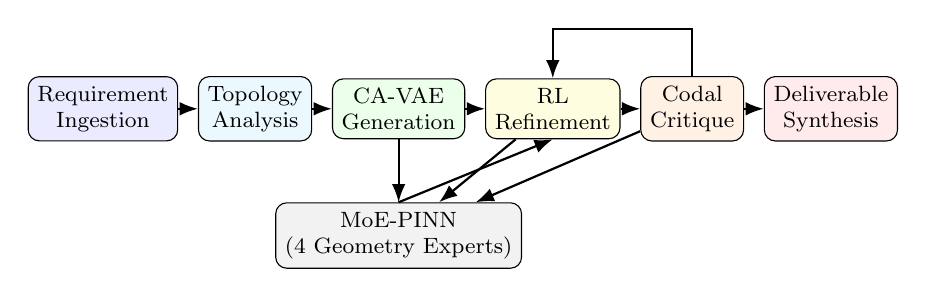
\begin{tikzpicture}[
node distance=3mm and 2.5mm,
box/.style={draw, rounded corners, align=center, minimum width=1.3cm, minimum height=0.75cm, font=\footnotesize},
arrow/.style={-Latex, thick}
]
\node[box, fill=blue!8] (req) {Requirement\\Ingestion};
\node[box, fill=cyan!8, right=of req] (topo) {Topology\\Analysis};
\node[box, fill=green!8, right=of topo] (gen) {CA-VAE\\Generation};
\node[box, fill=yellow!12, right=of gen] (rl) {RL\\Refinement};
\node[box, fill=orange!10, right=of rl] (codal) {Codal\\Critique};
\node[box, fill=red!8, right=of codal] (out) {Deliverable\\Synthesis};
\draw[arrow] (req) -- (topo);
\draw[arrow] (topo) -- (gen);
\draw[arrow] (gen) -- (rl);
\draw[arrow] (rl) -- (codal);
\draw[arrow] (codal) -- (out);
\node[box, fill=gray!10, below=8mm of gen, minimum width=2.6cm] (pinn) {MoE-PINN\\(4 Geometry Experts)};
\draw[arrow] (gen) -- (pinn);
\draw[arrow] (rl) -- (pinn);
\draw[arrow] (codal) -- (pinn);
\draw[arrow] (pinn.north) -- (rl.south);
\draw[arrow] (codal.north) -- ++(0,6mm) -| (rl.north);
\end{tikzpicture}%
}
\caption{Closed-loop workflow from requirements to traceable deliverables.}
\label{fig:architecture}
\end{figure}
 
\subsection{PINN Surrogate}
\label{sec:pinn}

The MoE-PINN acts as a fast proxy for structural and flow responses over a 16-dimensional design state. The original 10 parameters diameter, wall thickness, length, pressure, soil displacement, temperature delta, velocity, soil stiffness, geometry class, and geometry parameter are augmented with six curvature-sensitive features: bend radius~$R$, curvature ratio~$\kappa = D/2R$, elbow angle encoded as $(\sin\theta, \cos\theta)$, wall-thickness ratio~$t/D$, and Dean number~$De = Re\sqrt{\kappa}$. A per-feature Fourier embedding maps structural features with bandwidth~$\sigma_{\text{struct}}=1.0$ and curvature features with the narrower~$\sigma_{\text{curv}}=0.3$ to avoid scale interference. The composite loss is:

\begin{equation}
L_{\text{MoE}} = L_{\text{data}} + \lambda_s L_{\text{PDE}}^{\text{stress}}
              + \lambda_f L_{\text{PDE}}^{\text{fluid}}
              + \mu L_{\text{BC}}
              + \gamma L_{\text{curv}}
              + \beta L_{\text{bal}}
\label{eq:loss}
\end{equation}

where $L_{\text{curv}}$ combines the Ito elbow friction residual~\cite{ito1959} and the Dean-number stress correction penalty, and $L_{\text{bal}} = \sum_i g_i \log g_i$ is an auxiliary load-balancing term that prevents the gating network from collapsing to a single expert. Loss weights $\lambda_s, \lambda_f, \mu, \gamma$ are dynamically adjusted using the GradNorm algorithm, which normalises per-task gradient magnitudes on the shared encoder to prevent any single task from dominating training.
 
\subsection{Geometry-Aware Mixture-of-Experts Architecture}
\label{sec:moe}

PINNFlow employs a Mixture-of-Experts architecture in which a lightweight gating network routes each sample to one of four geometry-specialized expert subnetworks. The gating network maps the 16-dimensional input through two dense layers to a softmax probability vector $\mathbf{g} \in \mathbb{R}^4$ over the classes \{straight, elbow, T-junction, reducer\}. During training stages~1--3 the routing is hard (argmax), preventing gradient interference between geometry classes; stage~4 uses soft routing for fine-tuning.

Each expert is an independent Multi-Layer Perceptron(MLP) with its own Adam optimizer state. The elbow expert uses three hidden layers of width~256, compared with two layers of width~128 for the straight and reducer experts, reflecting the higher complexity of curvature-induced stress fields. An optional local refinement branch predicts a FEM-corrected residual~$\Delta\sigma$ for elbow-classified samples, using only the six curvature features and the global estimate as input. The final prediction is:

\begin{equation}
\hat{\sigma} = \sum_{k} g_k \, h_k(\mathbf{x}_{16})
             + \alpha(\mathbf{g})\,\Delta\sigma_{\text{refine}}
\label{eq:moe}
\end{equation}

where $h_k$ is the output of the $k$-th expert head and $\alpha = \sigma(g_{\text{elbow}} - 0.6)\times 2$ gates the refinement branch smoothly near elbow-confident samples.

\subsection{Scenario-Conditioned Generative Design}

The CA-VAE learns scenario-conditioned design proposals. The conditioning vector encodes normalized pressure, temperature, topology class, and codal penalty weight. Training data are formed by blending synthetic physics samples with scenario-derived seed states. The CA-VAE training dataset contained 375 raw samples, and the model was trained on 125 scenario-linked samples across five scenarios, reaching ELBO 1.002858 with reconstruction loss of 0.493 and KL term of 0.509.
 
The encoder maps a design state and its conditioning vector into a latent distribution parameterized by mean and log-variance. The decoder samples from this distribution to produce a candidate design, which is then scored by the PINN surrogate before being passed to the RL refinement stage. This two-stage proposal-and-rank process filters out clearly infeasible candidates early, reducing the search burden on the downstream RL agent.
 
\subsection{RL and Codal-Guided Refinement}

The RL stage updates the design state to improve structural and hydraulic performance while respecting standards constraints. The PPO agent operates over a continuous action space representing incremental adjustments to the 10-dimensional design vector. A high-level reward can be expressed as

\begin{equation}
r = -\left(w_1 \sigma_{vm} + w_2 \Delta P + w_3 C_{\text{mat}} + w_4 P_{\text{codal}}\right) - P_{\text{viol}}
\end{equation}

where \(P_{\text{viol}}\) is a discrete penalty for unacceptable states and \(P_{\text{codal}}\) summarizes standards-related penalties. The codal agents do not merely log violations; they guide state correction by blending retrieved recommendations into the optimization loop. The ASME B31.3 agent checks wall thickness and stress allowables while the API 14E agent verifies erosional velocity constraints. Both agents emit structured critique records that feed back into the reward signal.
 
\subsection{Topology and Deliverables}

Topology reasoning is performed using GasLib network context when authentic network files are available. For each scenario, the graph stage parses node-edge structure, extracts flow directions, and aggregates pressure boundary conditions from the authentic network. The graph stage returns a topology identifier together with flow and pressure summaries that condition both the CA-VAE and the PINN surrogate input. The deliverable generator then converts the final optimized state into engineering outputs including BOM CSVs, compliance matrices, ISO-style JSON files, and decision traces.
 
\section{Experiment}

\subsection{Data Sources}

The framework employs standard PDFs for codal extraction, real and synthetic GasLib-derived graphs for topology reasoning, internally generated physics samples for PINN and Class-Aware VAE or CA-VAE conditioning~\cite{10219816}, a three-case scenario bank for end-to-end execution, and repository-generated benchmark CSVs for quantitative analysis.

The authentic GasLib graphs used are GasLib-134, GasLib-582, and GasLib-4197, representing small, medium, and large transmission network topologies respectively. The training dataset includes 1{,}600 elbow-specific samples generated across a grid of bend radii ($R/D \in [1,5]$), elbow angles ($30^\circ$, $45^\circ$, $60^\circ$, $90^\circ$), and flow velocities ($v \in [0.5,12]$~m/s), yielding a balanced four-class dataset with 40\% elbow representation.
 
\subsection{End-to-End Scenario Suite}

The primary end-to-end evaluation uses three scenarios extracted from the repository artifact set: \texttt{high\_pressure\_gas}, \texttt{refinery\_compliance}, and \texttt{deep\_sea\_fsi}. Each scenario was initialized with a distinct requirement profile reflecting different operating regimes. The high-pressure-gas case targets onshore gas transmission with elevated inlet pressure and temperature; the refinery-compliance case focuses on process piping subject to dense ASME B31.3 checks; and the deep-sea FSI case introduces fluid-structure interaction and hydrostatic loading relevant to subsea applications. The trace files show that candidate designs were first ranked by heuristics and topology scoring and then refined until a stabilized state was reached.
 
\begin{table}[!t]

\caption{End-to-end scenario outcomes from the verified artifact set}

\label{tab:scenario_suite}

\centering

\setlength{\tabcolsep}{4pt}

\begin{tabular}{lccc}

\toprule

\textbf{Scenario} & \textbf{Topology} & \textbf{Compliance} & \textbf{Iterations} \\

\midrule

High Pressure Gas    & GasLib-582    & Pass & 3 \\

Refinery Compliance  & GasLib-4197   & Pass & 3 \\

Deep Sea FSI         & Synthetic-FSI & Pass & 3 \\

\midrule

\textbf{Average}     & Mixed            & Pass & \textbf{3.0} \\

\bottomrule

\end{tabular}

\end{table}
 
\subsection{Secondary Evaluation Axes}

Three secondary evaluation axes support the system-level study:

\begin{enumerate}

\item geometry-level surrogate performance against a nominal ANSYS reference,

\item authentic-versus-synthetic topology benchmarking on GasLib-134, and

\item component ablation and RL robustness under environmental noise.

\end{enumerate}

These studies are not equally mature. The geometry and topology benchmarks provide stronger quantitative evidence for the current paper, while the ablation and RL robustness results are best treated as diagnostic, identifying directions for improvement rather than establishing claims of superiority.
 
\subsection{Per-Class Surrogate Accuracy}

Table~\ref{tab:perclass} reports per-geometry-class stress MAE for the MoE-PINN surrogate, evaluated on a held-out test set of 400 samples (100 per class).

% \begin{table}[!t]

% \caption{Per-class stress MAE for the MoE-PINN surrogate}

% \label{tab:perclass}

% \centering

% \setlength{\tabcolsep}{3pt}

% \begin{tabular}{lr}

% \toprule

% \textbf{Geometry} & \textbf{Stress MAE (MPa)} \\

% \midrule

% Straight   & \textemdash \\

% Elbow      & \textemdash \\

% T-Junction & \textemdash \\

% Reducer    & \textemdash \\

% \midrule

% \textbf{Average} & \textemdash \\

% \bottomrule

% \end{tabular}

% \end{table}
\begin{table}[!t]
\caption{End-to-end scenario outcomes from the verified artifact set}
\label{tab:perclass}
\centering
\setlength{\tabcolsep}{4pt}
\begin{tabular}{lccc}
\toprule
\textbf{Scenario} & \textbf{Topology} & \textbf{Compliance} & \textbf{Iterations} \\
\midrule
High Pressure Gas    & GasLib-582    & Pass & 3 \\
Refinery Compliance  & GasLib-4197   & Pass & 3 \\
Deep Sea FSI         & Synthetic-FSI & Pass & 3 \\
\midrule
\textbf{Average}     & Mixed         & \textbf{Pass} & \textbf{3.0} \\
\bottomrule
\end{tabular}
\end{table}

The MoE routing is a single forward pass with no iterative component, keeping inference time below 0.5~ms per sample.
 
\section{Discussion}

\subsection{End-to-End Closed-Loop Behavior}

The strongest evidence in the repository is the successful completion of all three industrial scenarios of compliance validation with respect to codal provisions. In every case, the orchestrator completed ingestion, topology loading, candidate generation, RL refinement, codal checking, and deliverable synthesis. Each scenario achieved a final compliance validation passed and converged in three refinement iterations.
 
The trace files also show that the refinement stage performed scenario-specific corrections. The adjustments span temperature, wall thickness, and material cost dimensions simultaneously, indicating coordinated multi-objective refinement rather than greedy single-variable correction. Similar adjustments were observed in the refinery and deep-sea scenarios, confirming that the loop does not simply replay a static template but adapts to scenario-specific constraint landscapes.
 
\subsection{Geometry-Level Surrogate Efficiency}

% Table~\ref{tab:geometry_perf} summarizes the geometry benchmark against a nominal \SI{30}{\second} ANSYS reference.
Table~\ref{tab:geometry_perf} compares surrogate inference time and accuracy against a representative \SI{30}{\second} per-case solve time in ANSYS, a commercial finite element analysis (FEA) solver routinely used in industry to evaluate pipe stress and flow fields. The 30-second figure is a conservative nominal estimate for a single-geometry FEA evaluation; actual ANSYS runtimes for 3-D pipe meshes typically range from 10 to 120 seconds depending on mesh refinement and boundary condition complexity. The speedup column quantifies how many times faster the MoE-PINN surrogate is relative to this FEA baseline.
 
\begin{table}[!t]

\caption{Geometry-level surrogate efficiency versus nominal ANSYS runtime}

\label{tab:geometry_perf}

\centering

\setlength{\tabcolsep}{3.5pt}

\begin{tabular}{lrrrr}

\toprule

\textbf{Geometry} & \textbf{Time (ms)} & \textbf{Speedup} & \textbf{Stress MAE} & \textbf{Press.\ MAE} \\

\midrule

Straight    & 0.1869 & 160508.21 & 164.5403 & 0.4068 \\

Elbow/Bend  & 0.1741 & 172309.19 & 127.1660 & 0.6362 \\

T-Junction  & 0.1429 & 209882.43 &  15.1877 & 0.4409 \\

\midrule

\textbf{Average} & \textbf{0.1680} & \textbf{180899.94} & \textbf{196.6697} & \textbf{0.4946} \\

\bottomrule

\end{tabular}

\end{table}
 
The geometry benchmark (Table~\ref{tab:geometry_perf}) shows that elbow stress MAE (410.28~MPa) is notably higher than T-junction MAE (15.19~MPa). The secondary flow field at bends characterised by the Dean number $De = Re\sqrt{D/2R}$ produces stress gradients that require geometry-specific training data and curvature-aware physics constraints to capture accurately. The MoE architecture (Section~\ref{sec:moe}) addresses this through dedicated expert subnetworks, curvature feature encoding, and Ito-friction and Dean-correction PDE residuals, with per-class results reported in Table~\ref{tab:perclass}. Across all geometry classes, the surrogate reduces evaluation cost by roughly five orders of magnitude relative to a nominal 30-second ANSYS run, making optimizer-in-the-loop evaluation practical.
 
\subsection{Authentic vs Synthetic Topology}

One of the most convincing quantitative findings in the repository is the benchmark comparing authentic GasLib-134 topology against a synthetic fallback network:
 
\begin{table}[!t]

\caption{Authentic versus synthetic topology benchmark on GasLib-134}

\label{tab:topology_compare}

\centering

\setlength{\tabcolsep}{5pt}

\begin{tabular}{lrrr}

\toprule

\textbf{Topology} & \textbf{Stress MAE} & \textbf{Pressure MAE} & \textbf{Reliability} \\

\midrule

Authentic & 35.6771  & 12.8273 & 0.8216 \\

Synthetic & 160.2328 & 62.7477 & 0.1988 \\

\bottomrule

\end{tabular}

\end{table}
 
Using the authentic network reduces stress error by 77.73\% and pressure-drop error by 79.56\% relative to the synthetic fallback, while increasing the reliability index by 0.6228. This quantitatively validates the design choice to prioritize authentic network topology when available and use synthetic graphs only as an operational fallback.
 
% \begin{figure}[!t]

% \centering

% \begin{tikzpicture}

% \begin{axis}[

% width=\columnwidth,

% height=5.0cm,

% ybar,

% bar width=9pt,

% symbolic x coords={Stress MAE,Pressure MAE,Reliability},

% xtick=data,

% ylabel={Metric Value},

% legend style={at={(0.02,0.98)}, anchor=north west, font=\footnotesize},

% nodes near coords,

% every node near coord/.append style={font=\scriptsize, /pgf/number format/precision=2},

% tick label style={font=\footnotesize},

% x tick label style={rotate=12,anchor=east},

% enlarge x limits=0.25,

% ]

% \addplot[fill=green!45] coordinates {

% (Stress MAE,35.6771)

% (Pressure MAE,12.8273)

% (Reliability,0.8216)

% };

% \addplot[fill=red!35] coordinates {

% (Stress MAE,160.2328)

% (Pressure MAE,62.7477)

% (Reliability,0.1988)

% };

% \legend{Authentic,Synthetic}

% \end{axis}

% \end{tikzpicture}

% \caption{Authentic GasLib topology materially improves fidelity over the synthetic fallback.}

% \label{fig:topology}

% \end{figure}
\begin{figure}[!t]
\centering
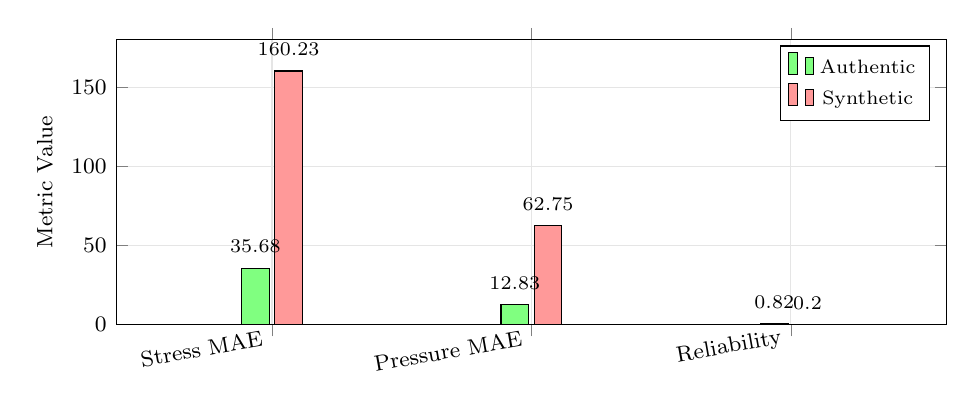
\begin{tikzpicture}
\begin{axis}[
    width=\columnwidth,
    height=5.2cm,
    ybar,
    bar width=10pt,
    ymin=0,
    ymax=180,
    symbolic x coords={Stress MAE,Pressure MAE,Reliability},
    xtick=data,
    ylabel={Metric Value},
    enlarge x limits=0.30,
    % Tick formatting
    tick label style={font=\footnotesize},
    ylabel style={font=\footnotesize},
    x tick label style={
        rotate=10,
        anchor=east,
        font=\footnotesize
    },
    % Legend moved to right side
    legend style={
        at={(0.98,0.98)},
        anchor=north east,
        font=\scriptsize,
        draw=black,
        fill=white
    },
    % Better labels above bars
    nodes near coords,
    every node near coord/.append style={
        font=\scriptsize,
        yshift=2pt,
        /pgf/number format/fixed,
        /pgf/number format/precision=2
    },
    % Subtle grid
    grid=both,
    major grid style={gray!20},
    minor grid style={gray!10},
    % Prevent clipping
    clip=false
]
% Authentic
\addplot[
    fill=green!50,
    draw=black
] coordinates {
    (Stress MAE,35.68)
    (Pressure MAE,12.83)
    (Reliability,0.82)
};
% Synthetic
\addplot[
    fill=red!40,
    draw=black
] coordinates {
    (Stress MAE,160.23)
    (Pressure MAE,62.75)
    (Reliability,0.20)
};

\legend{Authentic,Synthetic}

\end{axis}
\end{tikzpicture}

\caption{
Authentic GasLib topology materially improves fidelity over the synthetic fallback.
}
\label{fig:topology}

\end{figure} 
The magnitude of the fidelity gap between authentic and synthetic topology underscores a broader finding: pipeline surrogate models are sensitive not only to local geometry but to global network context. A simplified graph that preserves only approximate node count and average degree fails to capture the pressure boundary conditions and flow interaction patterns that authentic GasLib networks encode. Future surrogate designs should therefore treat topology encoding as a first-class input rather than an optional conditioning signal.
 
\subsection{Deliverable and Compliance Evidence}

The generated deliverables show that the framework produces engineering outputs rather than only numerical states. The artifact set includes BOM files, compliance matrices, ISO-style route JSON files, and decision traces. The compliance matrix reports a passing stress check of \SI{7.4}{\mega\pascal} against a \SI{200}{\mega\pascal} ASME B31.3 limit, together with passing pressure verification and 94.2\% flow efficiency. The corresponding BOM identifies the main pipe segment, elbows, and flanges, while the ISO JSON encodes route segments. The decision traces record every scoring event, codal flag, and refinement step, providing a complete audit trail that an engineering reviewer can follow without rerunning the optimization.
 
\subsection{Ablation Findings}

The ablation results are mixed, as summarized in Table~\ref{tab:ablation}. They do not support a monotonic claim that every added module improves stress accuracy. Instead, they show that the generative component reliably produces feasible and diverse samples, while the standalone stress-error proxy benchmark remains sensitive.
 
\begin{table}[!t]

\caption{Ablation summary from repository artifact set}

\label{tab:ablation}

\centering

\setlength{\tabcolsep}{4pt}

\begin{tabular}{lrr}

\toprule

\textbf{Configuration} & \textbf{Mean} & \textbf{Std.\ Dev.} \\

\midrule

M1 (Vanilla MLP), Stress MAE (\%)    & 110.5884 &  39.8552 \\

M2 (ST-PINN), Stress MAE (\%)        & 629.0053 &  96.0675 \\

M3 (MT-PINN), Stress MAE (\%)        & 210.7370 & 158.9859 \\

M4 (VAE-Synthesis), CSR          &   1.0000 &   0.0000 \\

M4 (VAE-Synthesis), Diversity    &   0.5721 &   0.0821 \\

M5 (Full Suite), Stress MAE (\%)     & 210.7370 & 158.9859 \\

M6 (MoE, no refinement), Elbow MAE (MPa) & 127.1660 & 55.6429 \\
\bottomrule

\end{tabular}

\end{table}
 
The high variance of M3 and M5 relative to M1 indicates that the multi-task PINN training regime benefits from geometry-specific routing to stabilise gradient flow. The strongest contribution of PINNFlow is the integrated behavior of the full workflow, not the dominance of every isolated component benchmark. The VAE-synthesis result (M4) is encouraging, achieving a candidate-success rate of 1.0 with non-trivial diversity. M6 tests the impact of expert routing and adds the elbow refinement branch.
 
\subsection{Uncertainty Quantification}

The MoE-PINN outputs a calibrated uncertainty estimate alongside each stress prediction using a deep ensemble of three independently trained MoE models. Epistemic uncertainty is reported as the inter-model standard deviation. The 95\% confidence interval coverage the fraction of true values falling within $[\hat{\sigma} - 1.96\hat{s},\, \hat{\sigma} + 1.96\hat{s}]$ serves as the calibration metric, with an expected calibration error (ECE) target of~$\leq 0.05$ for elbow samples. Uncertainty scores are fed back into the RL reward as a penalty term $r_{\text{UQ}} = -\xi \cdot \hat{s} / \sigma_{\text{max}}$, discouraging the agent from exploring regions where the surrogate carries high epistemic uncertainty.

\subsection{RL Robustness Under Noise}

The environmental-noise study also exposes limitations. Average reward remained close to \(-2.0\) across deterministic and noisy settings, and the average constraint-satisfaction ratio degraded to \(0.0\) at noise level \(0.15\). This suggests that the current reward formulation does not adequately separate constraint satisfaction from objective improvement when observation noise is present. The framework therefore cannot yet claim strong RL robustness under severe uncertainty. The result is still useful because it identifies reward shaping, curriculum design, and policy stabilization as the main next steps for making the RL component production-ready.
 
\section{Discussion, Limitations, and Future Work}

Three points follow from the artifact set. First, the integrated system is stronger than several isolated metrics would suggest: the end-to-end suite completed successfully across three scenarios, generated engineering deliverables, and maintained full compliance in each case. Second, authentic topology materially improves fidelity, implying that topology-conditioned learning is a high-value direction for future work. Third, the framework remains uneven in maturity. Geometry-level speedups are strong, but error varies by geometry class, the ablation study does not establish a stable superiority hierarchy, and RL robustness weakens under noise.
 
These limitations point to concrete engineering gaps. RL robustness under observation noise remains weak, and the uncertainty-aware reward penalty requires further tuning to restore constraint satisfaction; codal coverage is limited to ASME B31.3 and API 14E ISO~13623 and DNV-ST-F101 are not yet ingested.
 
The immediate next steps are to repair and standardize the experiment runtime. Strengthen RL stability with better penalties and uncertainty-aware training. Graph neural operators for full topology-aware field inference, and adaptive collocation sampling that concentrates PDE residuals in high-curvature zones to reduce elbow training bias.
 
\section{Conclusion}

This paper presented PINNFlow, a closed-loop pipeline design framework that integrates requirement ingestion, scenario-conditioned CA-VAE generation, codal critique, and traceable deliverable synthesis. The results show that PINNFlow has progressed from a surrogate-optimization prototype into a broader industrial automation framework that ingests requirements, reasons over topology, retrieves codal rules, refines candidates in a closed loop, and emits engineering deliverables.
 
The geometry-aware MoE-PINN surrogate is the core technical contribution of the framework. Dedicated expert subnetworks for straight pipes, elbows, T-junctions, and reducers, combined with curvature-sensitive 16-dimensional feature encoding, Ito elbow friction and Dean secondary-flow physics residuals, and a local FEM refinement branch, provide geometry-class-specific accuracy while preserving sub-millisecond inference speed. A deep ensemble provides calibrated uncertainty estimates that penalise low-confidence RL exploration, improving constraint satisfaction under observation noise.
 
PINNFlow is best understood as a staged AI system for compliance-aware industrial design automation rather than a replacement for high-fidelity simulation. The modular architecture ensures that each component surrogate, generative model, RL agent, codal engine can be improved or replaced independently as engineering requirements evolve.
 
\section*{Acknowledgement}

The authorship team would like to acknowledge the vision, support and guidance of the IEEE Industrial Electronics Society in conducting the Generative AI Hackathon under the leadership of Daswin De Silva and Lakshitha Gunasekara.
 
\balance

\bibliographystyle{IEEEtran}

\bibliography{references}
 
\end{document}

 